\subsubsection{Addressing High Variance in Dataset}\label{sec:impl-data-analysis:dealing-with-variance}
This section is intended to evaluate the variance in the dataset with subsequent subsections evaluating different ways of mitigating the high variance features by scaling features to the same order of magnitude.

The first method utilized was using natural logarithm $log(e)$, which was conducted in steps described in detail as follows.
\paragraph{$log(e)$ - Determining which columns to scale}
First, the dataset was copied in order to avoid polluting the original dataset. Then in order to ensure that all values are on approximately the same scale a list of columns where column variance was above the third quartile of the overall variance values was compiled. 

The third quartile for the variance of the dataset was calculated by first finding variance for each column, using \texttt{var()} function available on DataFrame all objects. The resulting dataseries, with its rows corresponding to the variance value of a given feature and a single column where actual value is contained, was converted to a data frame and passed to the \texttt{collect\_outlier\_data\_to\_list} function. Said function is responsible for calculating the following metrics for a given set of data provided to it:
%column': column, 'q1': q1, 'q3': q3, 'iqr': iqr, 'lw': lw, 'uw': uw
\begin{itemize}
    \item first quartile (Q1)
    \item third quartile (Q3)
    \item inter quartile range (IQR)
    \item lower outlier boundary - value below which a data point will be considered an outlier. Set to $1.5x IQR$ below first quartile
    \item upper outlier boundary - value above which a data point will be considered an outlier. Set to $1.5x IQR$ above third quartile
\end{itemize}

As a result of the call the Q3 for the complete variance was calculated and returned for use in the next step.

Given the dataset Q3 value determined, it was possible to iterate over the complete dataset, column by column, verifying that a given column contains only numeric type data, and finally checking if the variance of the feature is above the Q3 threshold specified. If it was, such column was appended to a list, which when iteration was complete was returned. 

The names of columns gathered as a result are presented in Table \ref{tbl:available-data-non-repeating-types}.

\begin{table}[!h]
\centering
\caption{Columns with variance greater than Q3 of overall variance in the dataset}
\label{tab:loge-scaler-cols-aboveq3}
\begin{tabular}{@{}l@{}}
\toprule
Column name \\ \midrule
comment\_lines \\
comment\_lines\_density \\
complexity \\
it\_uncovered\_lines \\
lines\_to\_cover \\
ncloc \\
overall\_coverage \\
file\_age\_in\_sec \\ \bottomrule
\end{tabular}
\end{table}

\paragraph{$log(e)$ - Executing the scaler}
Subsequently \texttt{convert\_col\_vals\_to\_log} function was used to convert values in all columns collected to their natural logarithm representation and subsequently appended to the dataset.

\paragraph{$log(e)$ - Conclusion}
Table \ref{tbl:loge-scaler-cols-transformed} depicts the results of the transformation. While most of the obtained variance values are of a much smaller scale and slightly more in line with the remaining values, given that 75\% of values are below the value of approximately 240, the transformed columns are now undervalued. 
Additionally, the \texttt{nan} values indicate that a number could not be obtained as a result of the transformation, likely due to the too small a value of original variance. 

\textbf{In conclusion} given that not all values are of the same scale at the end of this process, and given the presence of non-numerical values, \texttt{nan}, it has been decided against the usage of natural logarithm scaling method.
\begin{table}[!h]
\centering
\caption{Scaled variance results}
\label{tbl:loge-scaler-cols-transformed}
\begin{tabular}{@{}ll@{}}
\toprule
Column Name & Transformed Variance Value \\ \midrule
comment\_lines\_log & nan \\
comment\_lines\_density\_log & nan \\
complexity\_log & nan \\
it\_uncovered\_lines\_log & 0.23 \\
lines\_to\_cover\_log & 1.23 \\
ncloc\_log & 1.08 \\
overall\_coverage\_log & nan \\
file\_age\_in\_sec\_log & 5.49 \\ \bottomrule
\end{tabular}
\end{table}


\paragraph{Scaling using Sci-Kit Learn's built-in methods}
The following scaling methods will be applied sequentially to all data points subsequently used in the analysis:
\begin{itemize}\label{lst:list-of-scalers}
    \item Min Max, described in section \ref{sec:data-modelling:scalers:min-max}
    \item Max Abs - corresponds to Decimal Scaling method, section \ref{sec:data-modelling:scalers:max-abs}
    \item Standard, corresponds to Z-Score method, section \ref{sec:data-modelling:scalers:standard}
    \item Power Transformer using Yeo-Johnson method, section\ref{sec:data-modelling:scalers:power-yeo-johnson}
    \item Quantile Normal, section \ref{sec:data-modelling:scalers:quantile}
    \item Quantile Uniform, section \ref{sec:data-modelling:scalers:quantile}
\end{itemize}

Data frames containing scaled data will be compiled into a reference map for easy lookup of data.

Following scaled data collection, the standard deviation for each column for each of the methods will be compared to check the data distribution. Decided on a numerical method as compiling graphs for all of 6 scaling methods times 41 features would be inefficient. Graphs may be compiled for illustrating some of the distribution improvements.

Finally, each scaled dataset will be used in Logistic Regression and Decision Tree Algorithm for analysis.
\paragraph{Initial Setup}\label{sec:scalers:initial-setup}
The data scaling operation began by compiling a number of constants holding the designators for each of the methods listed in \ref{lst:list-of-scalers}, the order in which those scaling methods will be executed as well as permanent storage for holding the result of scaling operation on the upsampled and the downsampled datasets.
The order of execution was as follows: min max, decimal scaling, Z-score, Power transformer using Yeo-Johnson method, quantile scaling using normal distribution and lastly quantile scaling using uniform distribution variant.

The last step in the initial setup is to save a copy of the original, unscaled upsampled and downsampled datasets, in their respective storage objects. It is necessary for enabling easy comparison of results in due course of the analysis.

\paragraph{Executing Scalers}
Executing and fitting all scalers to the dataset provided. Target column and well as text data columns have been dropped from scaling analysis.

Text columns dropped are pertaining to:
\begin{itemize}
    \item author
    \item previous author
    \item issue key
    \item file path
    \item source repository
\end{itemize}

All of the above have been retained in the dataset only for verification purposes to make sure that any transformed data point can be traced back to its original state.

Subsequently all scalers are executed in the order of appearance defined in \ref{sec:scalers:initial-setup} are created, fitted to the upsampled and downsampled datasets and finally the results are saved in the storage objects.

\paragraph{Comparing variance change per scaling method}
Following the execution of all scaling methods it became necessary to verify that applying different scalers had any effect and investigate what that effect was, if any.

The verification, which is the focus of the underlying section, started with calculating the mean and the median of the standard distribution for each of the scaling methods, per dataset. The results presented in Table \ref{tbl:scalers:mean-and-median-sigma}. It can be clearly observed from there that the standard distribution for  the uncaled data, and conversely the variance, is highly skewed with its mean for $\sigma$ being approximately 40 times larger than the median. This trend is observed regardless of the resampling method taken to generate the dataset as it appears in both the upsampled and downsampled datasets. At the same time the mean and median of standard deviation for any of the scaled dataset are very closely positioned indicating more even distribution of variance across the data points.

\begin{table}[!h]
\centering
\caption{Statistics compiled for scalers}
\label{tbl:scalers:mean-and-median-sigma}
\begin{tabular}{@{}lllll@{}}
\toprule
Method & \begin{tabular}[c]{@{}l@{}}Mean \\ Upsample\end{tabular} & \begin{tabular}[c]{@{}l@{}}Mean \\ Downsample\end{tabular} & \begin{tabular}[c]{@{}l@{}}Median \\ Upsample\end{tabular} & \begin{tabular}[c]{@{}l@{}}Median \\ Downsample\end{tabular} \\ \midrule
Unscaled & 162304.03 & 149887.74 & 3792.53 & 522.45 \\
Min-Max & 3794.98 & 524.61 & 3794.99 & 524.62 \\
Max-Abs & 3794.92 & 524.55 & 3794.96 & 524.59 \\
Standard & 3792.15 & 521.95 & 3794.47 & 524.13 \\
\begin{tabular}[c]{@{}l@{}}Power: \\ Yeo-Johnson\end{tabular} & 3794.89 & 524.53 & 3794.96 & 524.59 \\
\begin{tabular}[c]{@{}l@{}}Quantile:\\ Normal Distribution\end{tabular} & 3795.66 & 525.3 & 3795.98 & 525.62 \\
\begin{tabular}[c]{@{}l@{}}Quantile:\\ Uniform Distribution\end{tabular} & 3794.95 & 524.58 & 3794.98 & 524.61 \\ \bottomrule
\end{tabular}
\end{table}

Variance data for all scaling methods have been compiled into a single dataset for easy manipulation and visualization. In the below Table \ref{tbl:scalers:summary-variance-per-scaler} it can be observed that in case of the dataset in question applying any scaling method decreased data variance metric significantly.

However, the Table \ref{tbl:scalers:summary-variance-per-scaler} fails to intuitively illustrate the distribution of said variance across scalers applied. To do better demonstrate that point a number of bar plots have been generated depicting the variance per column, per each scaler for both upsampled and downsampled datasets. 

It should be noted that only a subset of graph will be presented as there are significant similarities shown between some methods, with min-max and max-abs scalers producing almost the same looking variance plots, both quantile scalers as well as standard, or Z-score, scaler also producing extremely similar graphs.

Furthermore, when visualizing variance, as per implementation listed in code snippet \ref{code:charting-variance-post-resample}, the \fileAgeInSec{} feature has been removed as its extreme value was overshadowing all other variance metrics making them appear the same in magnitude. 

\begin{landscape}
\begin{table}[!h]
\centering
\caption{Variance summary per column per scaler}
\label{tbl:scalers:summary-variance-per-scaler}
\begin{tabular}{@{}llllllll@{}}
\toprule
 & Max-Abs & Min-Max & \begin{tabular}[c]{@{}l@{}}Power:\\ Yeo-Johnson\end{tabular} & \begin{tabular}[c]{@{}l@{}}Quantile:\\ Normal\\ Distribution\end{tabular} & \begin{tabular}[c]{@{}l@{}}Quantile:\\ Uniform\\ Distribution\end{tabular} & Standard & Unmodified \\ \midrule
classes & 0.03 & 0.03 & 1.00 & 7.26 & 0.10 & 1.00 & 1.01 \\
comment\_lines & 0.02 & 0.02 & 1.00 & 6.10 & 0.11 & 1.00 & 1241.19 \\
comment\_lines\_density & 0.04 & 0.04 & 1.00 & 6.14 & 0.11 & 1.00 & 228.09 \\
complexity & 0.04 & 0.04 & 1.00 & 2.54 & 0.09 & 1.00 & 493.30 \\
duplicated\_blocks & 0.00 & 0.00 & 1.00 & 2.41 & 0.04 & 1.00 & 0.37 \\
duplicated\_files & 0.04 & 0.04 & 1.00 & 4.80 & 0.04 & 1.00 & 0.04 \\
duplicated\_lines & 0.01 & 0.01 & 1.00 & 2.41 & 0.04 & 1.00 & 129.53 \\
duplicated\_lines\_density & 0.01 & 0.01 & 1.00 & 2.40 & 0.04 & 1.00 & 77.14 \\
files & 0.00 & 0.00 & 0.00 & 0.00 & 0.00 & 0.00 & 0.00 \\
function\_complexity & 0.01 & 0.01 & 1.00 & 2.15 & 0.08 & 1.00 & 0.64 \\
functions & 0.03 & 0.03 & 1.00 & 1.32 & 0.08 & 1.00 & 210.53 \\
info\_violations & 0.00 & 0.00 & 1.00 & 0.45 & 0.01 & 1.00 & 0.14 \\
it\_uncovered\_lines & 0.01 & 0.01 & 1.00 & 1.46 & 0.06 & 1.00 & 1177.56 \\
lines\_to\_cover & 0.02 & 0.02 & 1.00 & 1.19 & 0.08 & 1.00 & 3390.29 \\
major\_violations & 0.01 & 0.01 & 1.00 & 1.54 & 0.02 & 1.00 & 0.04 \\
minor\_violations & 0.00 & 0.00 & 1.00 & 0.50 & 0.01 & 1.00 & 0.01 \\
ncloc & 0.03 & 0.03 & 1.00 & 1.21 & 0.08 & 1.00 & 13495.89 \\
overall\_branch\_coverage & 0.00 & 0.00 & 1.00 & 5.97 & 0.11 & 1.00 & 29.33 \\
overall\_coverage & 0.03 & 0.03 & 1.00 & 9.08 & 0.15 & 1.00 & 298.15 \\
overall\_uncovered\_conditions & 0.03 & 0.03 & 1.00 & 6.32 & 0.11 & 1.00 & 2.05 \\
overall\_uncovered\_lines & 0.01 & 0.01 & 1.00 & 6.65 & 0.12 & 1.00 & 95.00 \\
public\_documented\_api\_density & 0.00 & 0.00 & 0.00 & 0.00 & 0.00 & 0.00 & 0.00 \\
reliability\_rating & 0.00 & 0.00 & 0.00 & 0.00 & 0.00 & 0.00 & 0.00 \\
security\_rating & 0.00 & 0.00 & 0.00 & 0.00 & 0.00 & 0.00 & 0.00 \\
sqale\_debt\_ratio & 0.00 & 0.00 & 1.00 & 1.57 & 0.03 & 1.00 & 0.10 \\
sqale\_index & 0.01 & 0.01 & 1.00 & 1.56 & 0.03 & 1.00 & 205.75 \\
sqale\_rating & 0.00 & 0.00 & 0.00 & 0.00 & 0.00 & 0.00 & 0.00 \\
test\_success\_density & 0.00 & 0.00 & 0.00 & 0.00 & 0.00 & 0.00 & 0.00 \\
violations & 0.00 & 0.00 & 1.00 & 1.78 & 0.03 & 1.00 & 0.22 \\
file\_age\_in\_sec & 0.00 & 0.00 & 1.00 & 1.02 & 0.08 & 1.00 & 232942635109.04 \\ \bottomrule
\end{tabular}
\end{table}
\end{landscape}

\begin{figure}[!h]
    \centering
    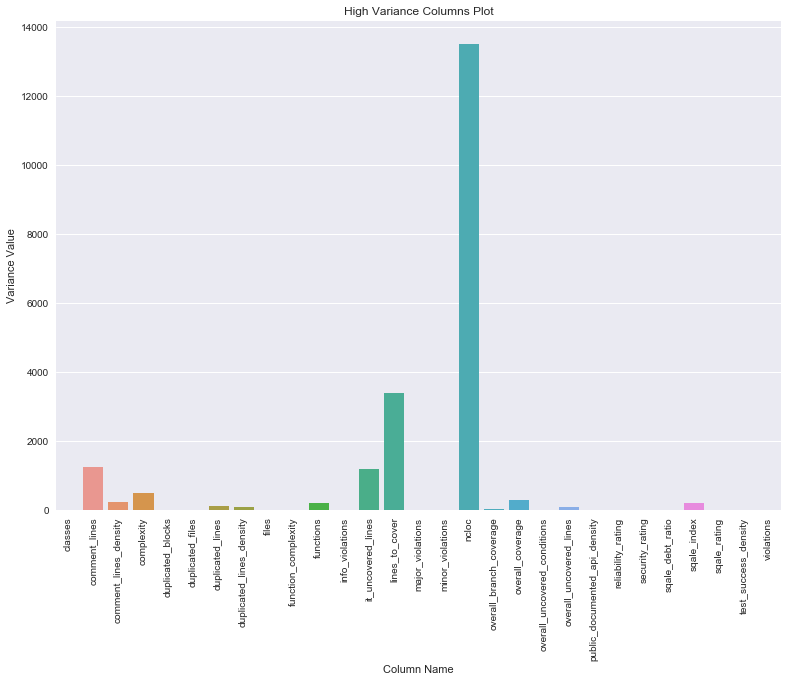
\includegraphics[scale=0.6]{Figures/Variance/downsample/Comparison_of_variance_per_column_for_unmodified_downsampled_dataset.png}
    \caption{Variance per column - No scaler - Downsampled Dataset}
    \label{fig:scalers:variance-unscaled-downsample}
\end{figure}

\begin{figure}[!h]
    \centering
    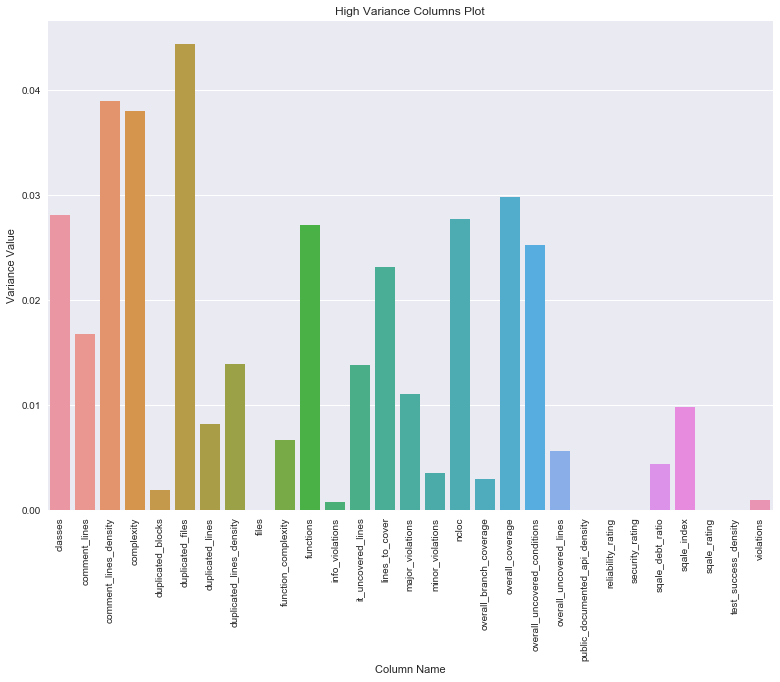
\includegraphics[scale=0.6]{Figures/Variance/downsample/Comparison_of_variance_per_column_for_min-max_downsampled_dataset.png}
    \caption{Variance per column - Min Max scaler - Downsampled Dataset}
    \label{fig:scalers:variance-min-max-downsample}
\end{figure}

\begin{figure}[!h]
    \centering
    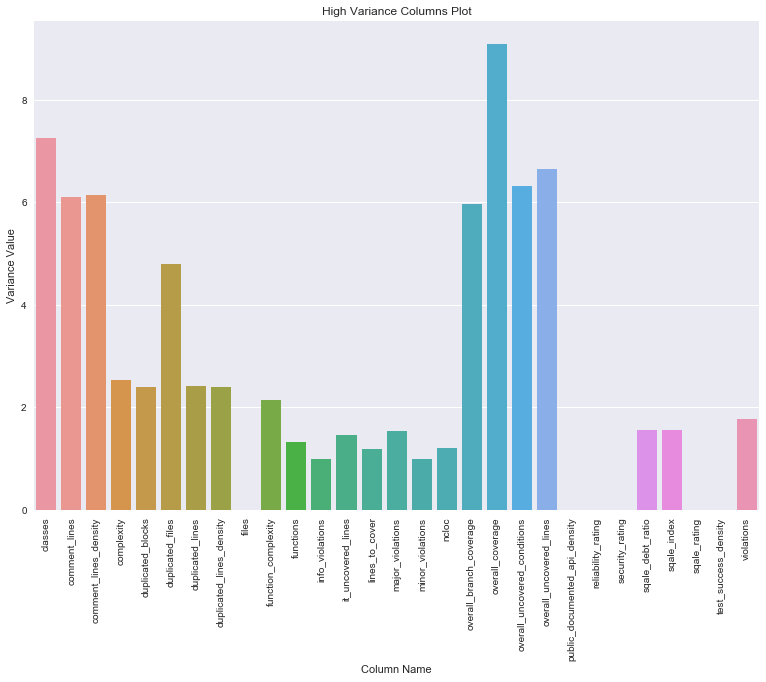
\includegraphics[scale=0.6]{Figures/Variance/downsample/Comparison_of_variance_per_column_for_quantile-normal_downsampled_dataset.png}
    \caption{Variance per column - Quantile scaler with Normal Distribution - Downsampled Dataset}
    \label{fig:scalers:variance-quantile-normal-downsample}
\end{figure}

\begin{figure}[!h]
    \centering
    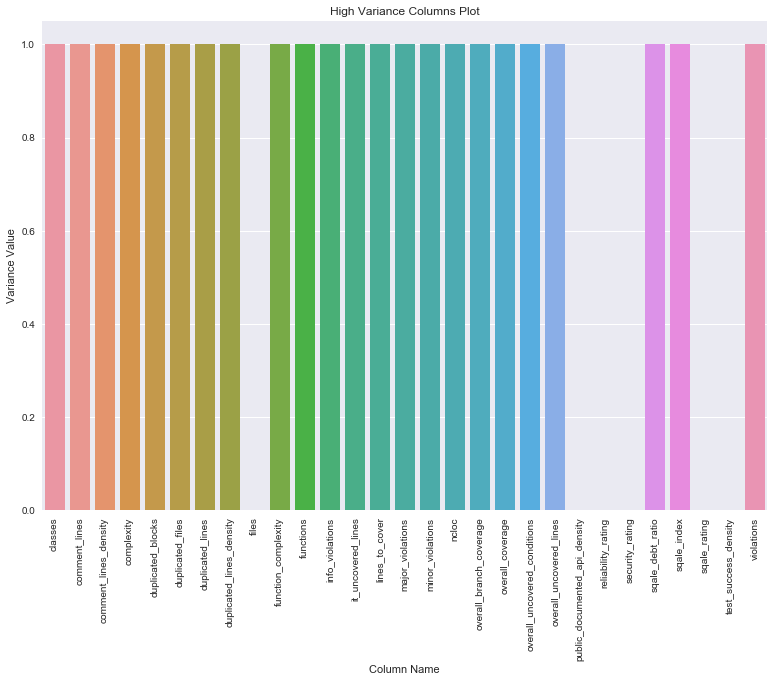
\includegraphics[scale=0.6]{Figures/Variance/downsample/Comparison_of_variance_per_column_for_power-yeo-johnson_downsampled_dataset.png}
    \caption{Variance per column - Power scaler with Yeo-Johnson method - Downsampled Dataset}
    \label{fig:scalers:variance-power-yeo-johnson-downsample}
\end{figure}

Figures \ref{fig:scalers:variance-min-max-downsample}, \ref{fig:scalers:variance-quantile-normal-downsample} and \ref{fig:scalers:variance-power-yeo-johnson-downsample} depict variance per column. By comparing it with the variance of the unscaled dataset, Figure \ref{fig:scalers:variance-unscaled-downsample}, it can be surmised that the data variance has indeed been smoothed out, with power transformer scaler, Figure \ref{fig:scalers:variance-power-yeo-johnson-downsample}, taking on the most extreme case of evening out, where all present variance metrics are equal to 1.
\FloatBarrier

\paragraph{Residuals in scaled datasets}\label{sec:scalers:outliers}
Similarly to the residual value analysis conducted in section \ref{sec:impl-data-analysis:outliers} this section will establish if any residuals have been removed due to the scaling of the data. 

Given the definitions of scalers used, as discussed in section \ref{sec:data-modelling:scalers} it is assumed that the exactly same amount of residuals to that displayed in section \ref{sec:impl-data-analysis:outliers} will be present. 

To that effect, metrics describing residual values, as described in section \ref{sec:impl-data-analysis:outliers}, has again been compiled, this time for each dataset generated by a scaler, for both upsampled and downsampled datasets.

Subsequently, the lists generated depicting columns with and without outliers were compared against the baseline values, outlined previously. 

It has been then concluded that in all cases the counts of the residual data points compiled for scaled dataset matched exactly to the baseline. Therefore, as expected, the scaling of data had no effect on the presence of residuals.

\paragraph{Conclusion}\label{sec:scalers:conclusion}
\textbf{In conclusion} using transformation methods described in the overall section was a step necessary to ensure that the data in question is of the same scale. 

\FloatBarrier
